% LaTeX Article Template
\documentclass[12pt]{article}
%% Other packages
\usepackage{amsmath}
\usepackage{amsthm}
\usepackage{titlesec}
\usepackage{soul}
\usepackage{tikz}
\usepackage{tikz-3dplot}
\usepackage{amssymb}
\usepackage{multicol}
\usepackage{float}
\usepackage{calc}
\usepackage{fancybox}
\usepackage{array}
\usepackage[shortlabels]{enumitem}
\usepackage{framed}
\usepackage{hyperref}
\newcolumntype{L}[1]{>{\raggedright\let\newline\\\arraybackslash\hspace{0pt}}m{#1}}
\newcolumntype{C}[1]{>{\centering\let\newline\\\arraybackslash\hspace{0pt}}m{#1}}
\newcolumntype{R}[1]{>{\raggedleft\let\newline\\\arraybackslash\hspace{0pt}}m{#1}}


%% Margins
\usepackage{geometry}
\geometry{verbose,letterpaper,tmargin=1in,bmargin=1in,lmargin=1in,rmargin=1in}

\newcommand{\menuchoice}[2]{{\ttfamily#1..#2}}
\newcommand{\dotdot}{..}

\usepackage{graphicx}

% Array vertical and horizontal stretch
% \def\arraystretch{1.5}%  1 is the default, change whatever you need
% \setlength{\tabcolsep}{12pt}

%\graphicspath{%
\graphicspath{{./figs/}}

%% Paragraph style settings
\setlength{\parskip}{\medskipamount}
\setlength{\parindent}{0pt}

%% Change itemize bullets
\renewcommand{\labelitemi}{$\bullet$}
\renewcommand{\labelitemii}{$\circ$}
\renewcommand{\labelitemiii}{$\diamond$}
\renewcommand{\labelitemiv}{$\cdot$}

%% Shrink section fonts
\titleformat*{\section}{\large\bf}
\titleformat*{\subsection}{\normalsize\it}
\titleformat*{\subsubsection}{\normalsize\bf}

% %% Compress the spacing around section titles
\titlespacing*{\section}{0pt}{1.5ex}{0.75ex}
\titlespacing*{\subsection}{0pt}{1ex}{0.5ex}
\titlespacing*{\subsubsection}{0pt}{1ex}{0.5ex}

%% amsthm settings
\theoremstyle{definition}
\newtheorem{problem}{Problem}
\newtheorem{example}{Example}
\newtheorem{mydef}{Definition}

%% Answer box macros
%% \answerbox{alignment}{width}{height}
\newcommand{\answerbox}[3]{%
  \fbox{%
    \begin{minipage}[#1]{#2}
      \hfill\vspace{#3}
    \end{minipage}
  }
}

%% \answerboxfull{alignment}{height}
\newcommand{\answerboxfull}[2]{%
  \answerbox{#1}{\textwidth}{#2} 
}

%% \answerboxone{alignment}{height} -- for first-level bullet
\newcommand{\answerboxone}[2]{%
  \answerbox{#1}{6.15in}{#2} 
}

%% \answerboxtwo{alignment}{height} -- for second-level bullet
\newcommand{\answerboxtwo}[2]{%
  \answerbox{#1}{5.8in}{#2}
}

%% \graphbox{xmin}{xmax}{ymin}{ymax}{scale}
\newcommand{\graphbox}[5]%[-5, 5, -5, 5, 0.33]
{
\begin{tikzpicture}
     [>=latex,scale=#5]
     
     % Coordinate axes
     \draw [->,very thick] (#1, 0) -- (#2, 0) node[right] {$x$};
     \draw [->,very thick] (0, #3) -- (0, #4) node[above] {$y$};
     
     % Grid
     \draw[step=1cm,thick,dotted] (#1,#3) grid (#2,#4);
   \end{tikzpicture}
   }


%% Redefine maketitle
\makeatletter
\renewcommand{\maketitle}{
  \noindent SA403 -- Networks \\

  \begin{center}\Large{\textbf{\@title}}\end{center}
}
\makeatother

% Set the beginning of a LaTeX document
\begin{document}

%\graphbox{-10}{3}{-5}{10}

\title{Lesson 3: Shortest-path Problems}

%\graphbox[10][10]

\maketitle


\section*{Notes}

Book acknowledgment:
\section*{Goals}
\begin{itemize}
\item Shortest path 
\end{itemize}




\section{Try it on your own}

\begin{center}
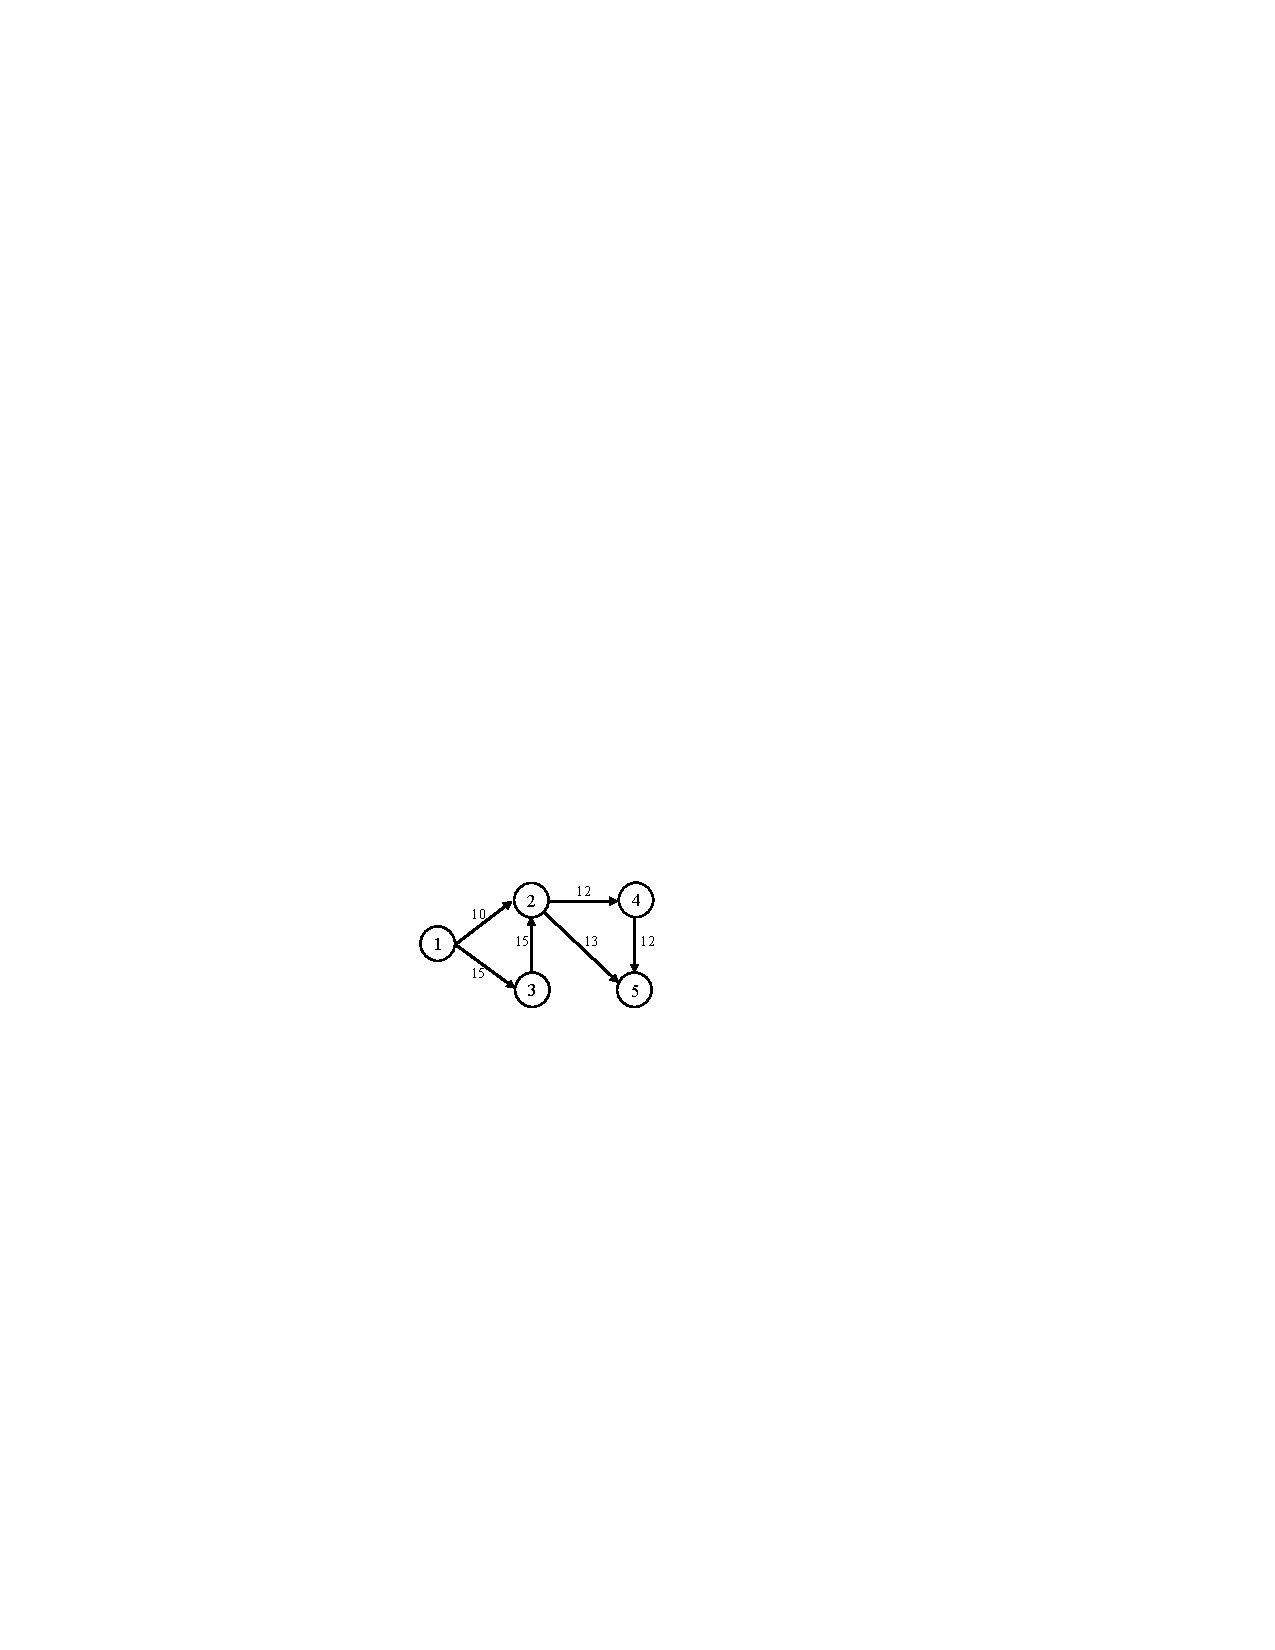
\includegraphics[width=5cm]{shortestpathexample1}
\end{center}

\begin{enumerate}[a.]

\item Determine a shortest path from 1 to 5.
\vfill
\item Determine a shortest path from 1 to every other node.
\vfill

\newpage
\begin{center}
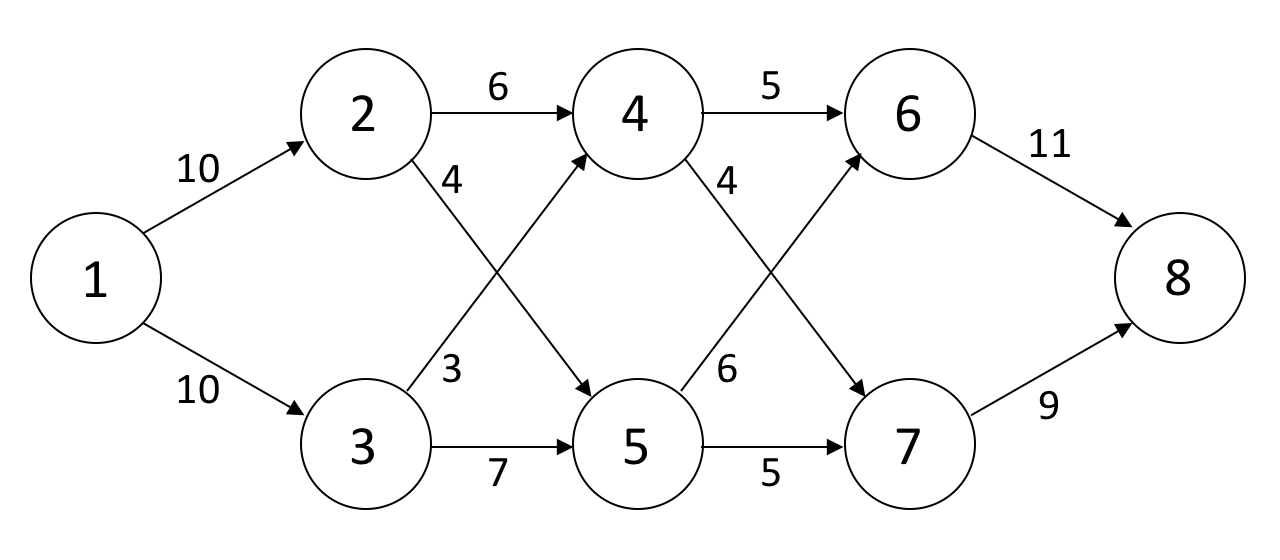
\includegraphics[width=10cm]{shortestpathexample2}
\end{center}

\item Determine a shortest path from 1 to 8.
\vfill
\item Determine a shortest path from 1 to every other node.
\vfill


\end{enumerate}

\newpage


\section{Problem Definition}

\begin{itemize}
\item Given a directed graph $G=(V,A)$, let $s$ be the source (origin) node and $t$ be the terminal (sink) node. 
\item Let $c_{ij}$ be the cost of traversing arc $(i,j) \in A$.
\end{itemize}

\textbf{Shortest path problem:} Determine the minimum cumulative cost path from $s$ to $t$.


How would you go about solving this on your own? (Given what you already know from previous courses.)

\vfill

\section{Dijkstra's Algorithm}

Dijkstra's algorithm is very similar to Prim's Algorithm in that we will keep track of which nodes are and are not included in a shortest path from $s$ to $t$. In doing so, we will actually build a shortest-path tree rooted at the source node $s$.

At each step of the algorithm, we will search for a node not yet in the shortest-path tree having a minimum distance from the source.

\vfill

\newpage

\textbf{Steps:}
\begin{enumerate}
	\item Initialize set $S = \emptyset$ that contains all the nodes currently in the shortest-path tree. If a node $i \in V$ is in the shortest-path tree, then we have successfully determined a shortest path from $s$ to $i$.

	\item Assign a minimum distance value $v_i$ to each node $i \in V$ in the graph. Initialize $v_i = \infty, \ \forall i \in V$. Set $v_s = 0$.

	\item While $S \subset V$:
	\begin{enumerate}
		\item Pick a node $u \in V \setminus S$ having a minimum distance value $v_u = \textrm{min} \{v_i: i \in V\setminus S\}$.
		\item Add $u$ to $S$. 
		\item Update the distance value for each adjacent node of $u$. For all $(u,w) \in A$, if $v_w > v_u + c_{uw}$, then set $v_w = v_u + c_{uw}$. 
	\end{enumerate}
\end{enumerate}

\newpage

\section*{Let's practice!}

Use Dijkstra's Algorithm to solve the two examples from earlier.

\begin{center}
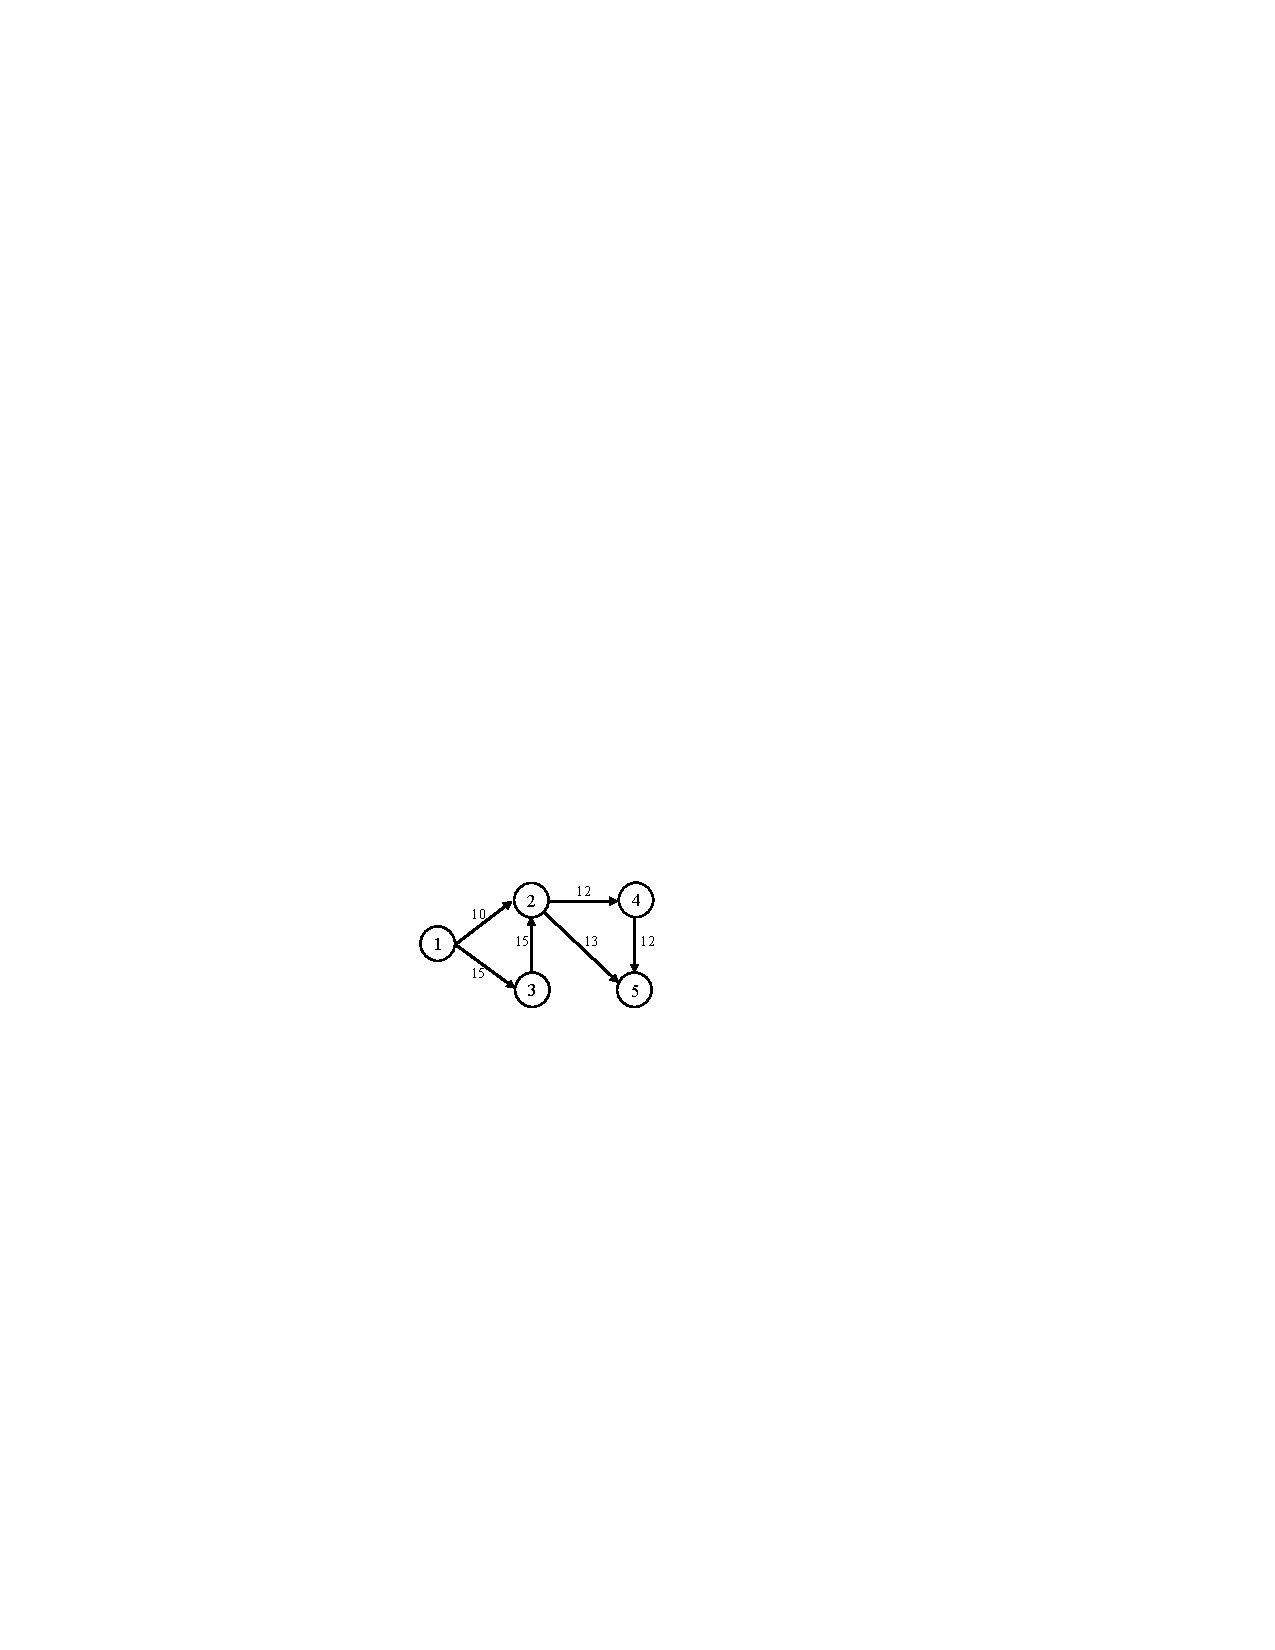
\includegraphics[width=5cm]{shortestpathexample1}
\end{center}
\vfill

\begin{center}
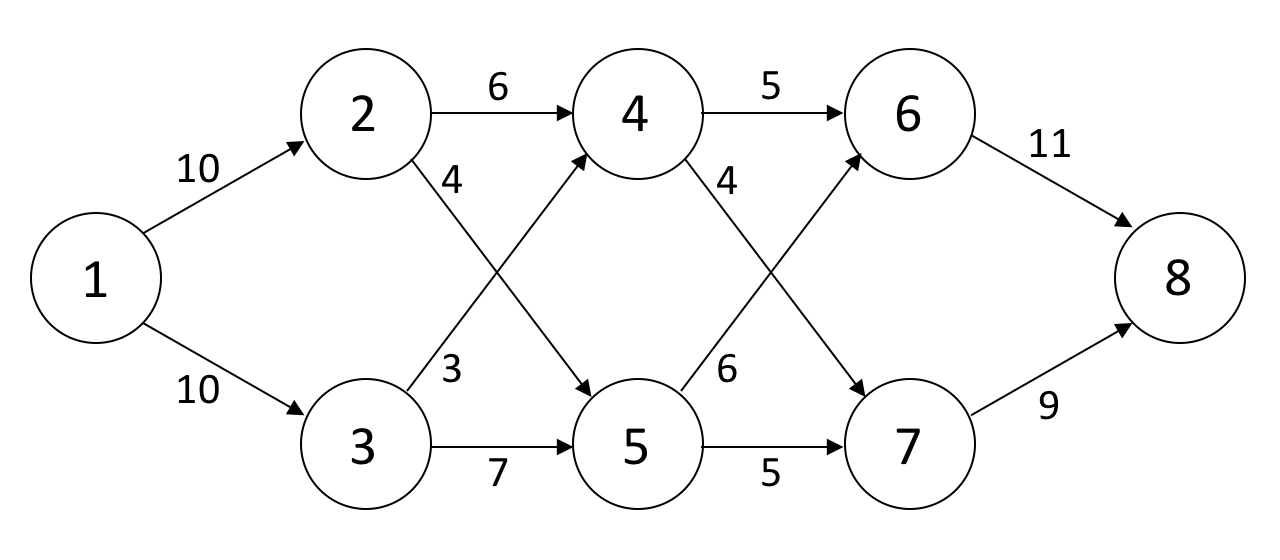
\includegraphics[width=10cm]{shortestpathexample2}
\end{center}

\vfill

\newpage

\section{What could go wrong?}

\begin{itemize}

\item The two examples from earlier all have positive arc costs. What could go wrong if some arcs have a negative cost?

\end{itemize}
\vfill
 
Use Dijkstra's Algorithm to determine the shortest path from $s$ to every other node in $V \setminus \{s\}$.

\begin{center}
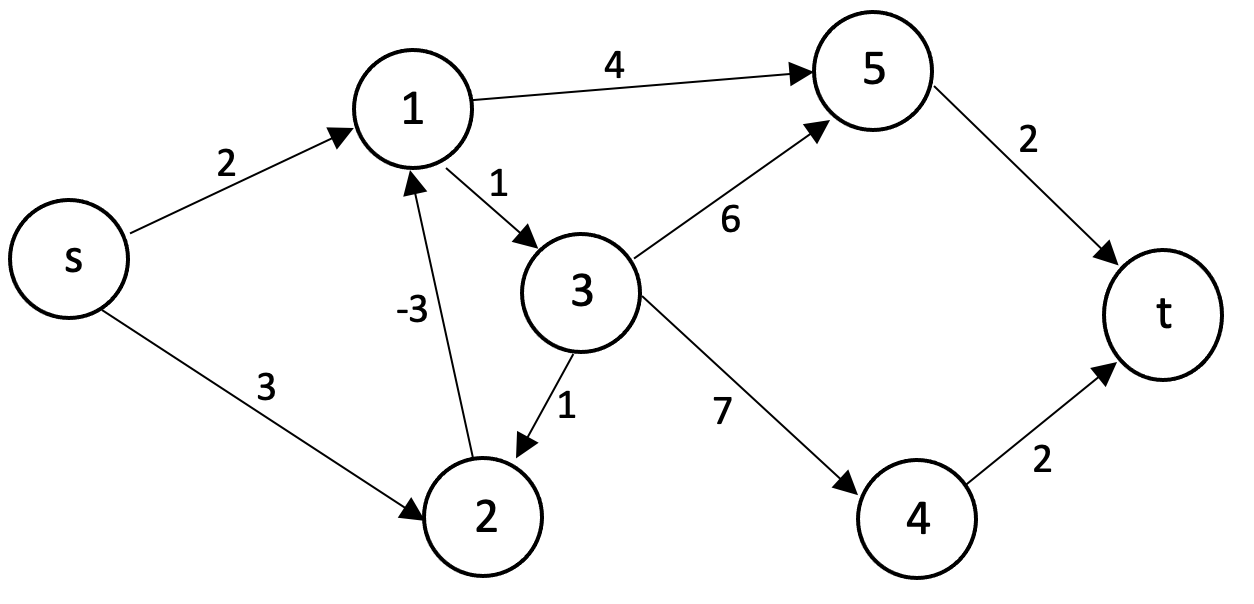
\includegraphics[width=10cm]{shortestpathnegativecycles}
\end{center}

\vfill


\newpage
\section{Bellman-Ford Algorithm}


The Bellman-Ford Algorithm is slightly slower than Dijkstra's Algorithm but more versatile because it is capable of handling graphs having negative arc costs. If a graph/network has a negative-cost cycle, then the Bellman-Ford Algorithm is able to detect and report it.

Like Dijkstra's Algorithm, the Bellman-Ford iteratively updates approximations to the minimum computed distance to each node in the network. Whereas Dijkstra's uses a greedy apporach that selects the \emph{closest} node that has not yet been added to the shortest-path tree set $S$, Bellman-Ford updates all edges at most $|V| - 1$ times. 

\textbf{Steps:}

\begin{enumerate}

\item Set $k = 0$, $v_s = 0$, and $v_i = \infty, \forall i \in V \setminus \{s\}$
\item While $k < |V| - 1$:
	\begin{enumerate}
		\item For all $(i,j) \in A$, if $v_j > v_i + c_{ij}$ and $v_i < \infty$, then set $v_j = v_i + c_{ij}$. 
		\item Set $k = k + 1$. 
	\end{enumerate}
\end{enumerate}

 \newpage
Use the Bellman-Ford Algorithm to determine the shortest path from $s$ to every other node in $V \setminus \{s\}$.

\begin{center}
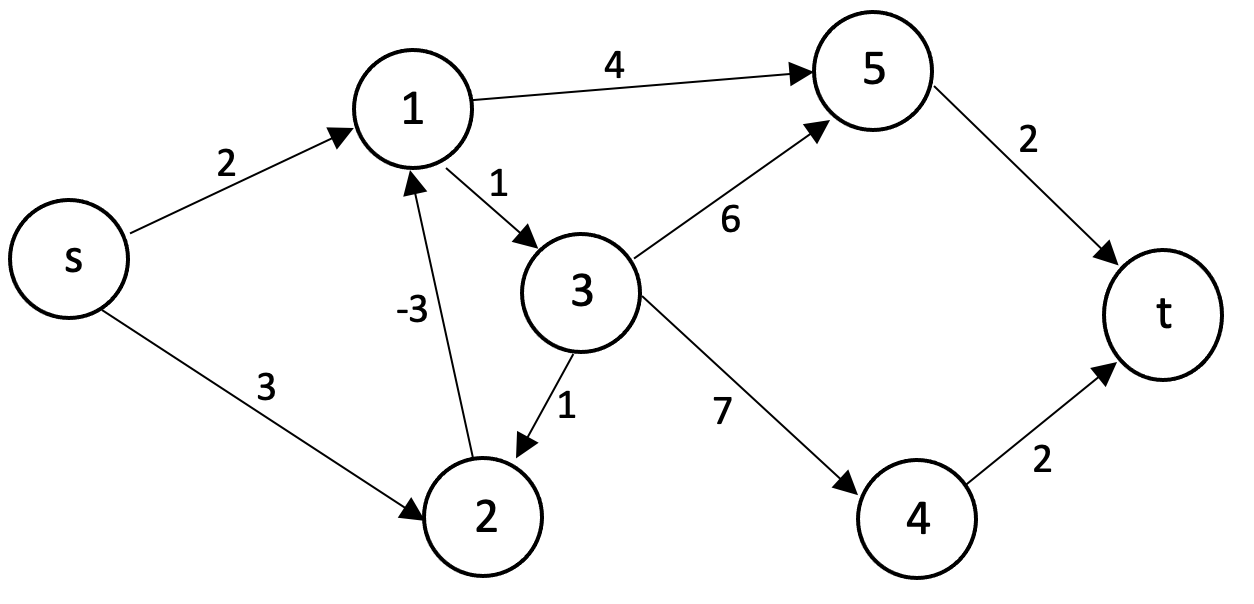
\includegraphics[width=10cm]{shortestpathnegativecycles}
\end{center}

\vfill


\newpage

\section{Running Time Analysis}

\begin{itemize}

\item What's the worst-case running time for Dijkstra's Algorithm?

\vfill

\item What's the worst-case running time for the Bellman-Ford Algorithm?

\vfill
\end{itemize}

\end{document}
